\documentclass[conference]{IEEEtran}
\IEEEoverridecommandlockouts

\usepackage{amsmath,amssymb,amsfonts}
\usepackage{graphicx}
\usepackage{booktabs}
\usepackage{multirow}
\usepackage{cite}
\usepackage[hidelinks]{hyperref}
\usepackage{array}
\usepackage{caption}
\usepackage{balance}
\usepackage{enumitem}
\usepackage{tikz}
\usetikzlibrary{positioning,arrows.meta,shapes.geometric,calc}
\setlength{\textfloatsep}{6pt}
\setlength{\abovecaptionskip}{4pt}
\setlength{\belowcaptionskip}{0pt}
\setlength{\dbltextfloatsep}{8pt}
\setlength{\intextsep}{6pt}
\renewcommand{\arraystretch}{1.08}
\setlist{nosep,leftmargin=1.2em}

\begin{document}

\title{Domain-Enhanced Mixture-of-Experts Adapter for\\
Parameter-Efficient Remote Sensing Image-Text Retrieval}

\author{\IEEEauthorblockN{Linyihan Zhang}
\IEEEauthorblockA{Maynooth International Engineering College, Fuzhou University}}

\maketitle

\begin{abstract}
Remote sensing image-text retrieval (RSITR) aims to match overhead images with natural language descriptions. Although CLIP-style vision-language pre-training provides strong cross-modal representations, directly transferring such models to RSITR remains challenging because remote sensing scenes contain large intra-class variation, complex spatial organization, and incomplete image-text correspondence. Meanwhile, full fine-tuning is computationally expensive, while conventional parameter-efficient transfer learning methods often rely on a single adaptation path and therefore have limited capacity to model heterogeneous remote sensing patterns. To address these issues, this paper proposes a Domain-Enhanced Mixture-of-Experts Adapter (DeMoE) built on a frozen CLIP backbone. The proposed method introduces Semantic Expert Adapters to model diverse scene semantics through sparse expert activation, and further employs a Domain-Guided Selection mechanism to stabilize expert routing under domain shift. Experiments show that DeMoE achieves strong retrieval performance while updating only a small number of parameters.
\end{abstract}

\begin{IEEEkeywords}
remote sensing image-text retrieval, CLIP, parameter-efficient transfer learning, mixture-of-experts, domain adaptation
\end{IEEEkeywords}

\section{Introduction}
Remote Sensing Image-Text Retrieval (RSITR) retrieves relevant remote sensing images from natural language queries and supports applications such as urban analysis, disaster response, and geographic information understanding~\cite{ref1,ref4}. Recent CLIP-style dual-encoder models have become a strong baseline for cross-modal retrieval because they project images and texts into a shared embedding space and enable efficient large-scale matching~\cite{ref3}. However, the direct transfer of natural-image pre-trained models to remote sensing scenes is still difficult.

The first challenge is \emph{domain discrepancy}. Remote sensing images are captured from an overhead viewpoint and usually contain large-scale layouts, dense object distributions, and complex background structures, which are different from the object-centric distributions of natural images~\cite{ref2,ref4}. The second challenge is \emph{high intra-class variation}. Even scenes with the same label may differ greatly in texture, scale, and spatial arrangement, making stable image-text alignment difficult~\cite{ref5}. The third challenge is \emph{efficient adaptation}. Full fine-tuning of a large vision-language model is expensive, but standard adapters or LoRA usually provide only one lightweight transformation path in each layer, which is insufficient for highly heterogeneous remote sensing data~\cite{ref7}. In addition, recent RSITR systems often benefit from stronger remote sensing pre-training, but such strategies usually introduce additional data and computational cost~\cite{ref6,ref10}.

Based on these observations, this work reformulates the adaptation problem as \emph{how to preserve the efficiency of a frozen backbone while increasing the flexibility of domain-specific feature transformation}. To this end, a Domain-Enhanced Mixture-of-Experts Adapter (DeMoE) is proposed. Instead of using one fixed adapter in each Transformer block, DeMoE introduces multiple lightweight experts and activates only the most relevant ones for each token. This design is inspired by sparse Mixture-of-Experts, which has shown strong capacity-efficiency trade-offs in large models~\cite{ref8,ref9}. In addition, a domain-guided routing signal is designed to make sparse expert selection more stable during transfer from natural-image pre-training to remote sensing data.

The main contributions are as follows:
\begin{enumerate}
    \item A parameter-efficient DeMoE framework is proposed for RSITR by inserting sparse expert adapters into a frozen CLIP backbone.
    \item A Semantic Expert Adapter (SEA) is designed to increase adaptation capacity for diverse remote sensing scene patterns.
    \item A Domain-Guided Selection (DGS) strategy is introduced to improve routing stability under cross-domain transfer.
    \item Experiments on RSICD verify the effectiveness of the proposed design in both overall retrieval performance and component-level ablation.
\end{enumerate}

\section{Method}
\subsection{Problem Formulation}
Given a training set $\mathcal{D}=\{(I_i,T_i)\}_{i=1}^{N}$, where $I_i$ denotes a remote sensing image and $T_i$ denotes its paired text description, RSITR learns a shared embedding space for bidirectional retrieval~\cite{ref1,ref4}. With a visual encoder $f_v(\cdot)$ and a text encoder $f_t(\cdot)$, the image and text embeddings are written as
\begin{equation}
\mathbf{v}_i=f_v(I_i), \quad \mathbf{t}_i=f_t(T_i).
\end{equation}
After $\ell_2$ normalization, the similarity score is computed by scaled cosine similarity~\cite{ref3}:
\begin{equation}
 s(I_i,T_j)=\tau\frac{\mathbf{v}_i^{\top}\mathbf{t}_j}{\|\mathbf{v}_i\|\,\|\mathbf{t}_j\|},
\end{equation}
where $\tau$ is a learnable temperature.

\subsection{Motivation of DeMoE}
Conventional parameter-efficient transfer learning updates only a small number of newly introduced parameters, which is attractive for RSITR because annotated remote sensing datasets are usually limited~\cite{ref7}. However, a single adapter path cannot adequately handle large semantic diversity. In practice, some tokens mainly describe local structures such as roads, ships, or tanks, while others capture broad scene layouts such as coastlines, harbors, or residential regions. This suggests that different semantic patterns should not share exactly the same adaptation path.

DeMoE follows this intuition. The frozen CLIP backbone preserves strong general multimodal priors, while a sparse mixture of lightweight experts provides additional domain-specific flexibility. Thus, the model remains efficient but gains stronger representational capacity for heterogeneous remote sensing scenes.

\begin{figure}[t]
\centering
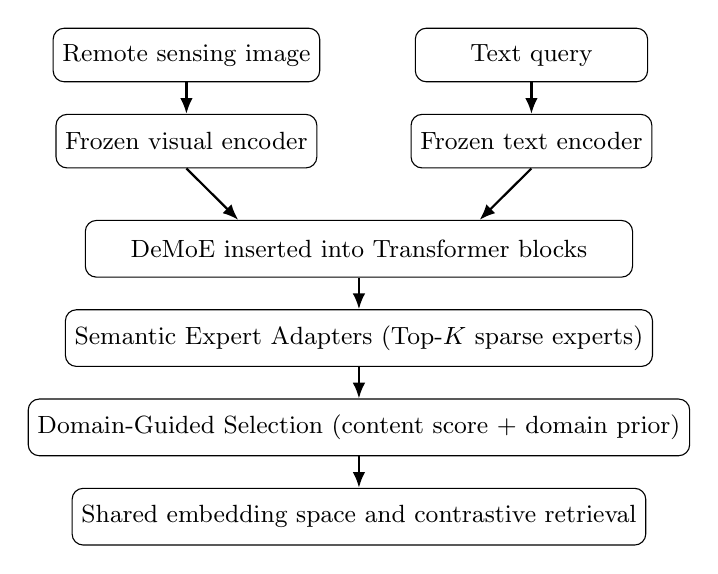
\begin{tikzpicture}[
node distance=4mm and 8mm,
block/.style={draw, rounded corners, align=center, minimum width=6.95cm, minimum height=0.72cm, font=\small},
smallblock/.style={draw, rounded corners, align=center, minimum width=2.95cm, minimum height=0.68cm, font=\small},
arr/.style={-{Latex[length=2mm,width=1.6mm]}, thick}
]
\node[smallblock] (img) {Remote sensing image};
\node[smallblock, right=12mm of img] (txt) {Text query};
\node[smallblock, below=of img] (ve) {Frozen visual encoder};
\node[smallblock, below=of txt] (te) {Frozen text encoder};
\node[block, below=10mm of $(ve)!0.5!(te)$] (demoe) {DeMoE inserted into Transformer blocks};
\node[block, below=of demoe] (sea) {Semantic Expert Adapters (Top-$K$ sparse experts)};
\node[block, below=of sea] (dgs) {Domain-Guided Selection (content score + domain prior)};
\node[block, below=of dgs] (ret) {Shared embedding space and contrastive retrieval};
\path (demoe.north west) -- (demoe.north east) coordinate[pos=0.28] (dleft) coordinate[pos=0.72] (dright);
\draw[arr] (img) -- (ve);
\draw[arr] (txt) -- (te);
\draw[arr] (ve.south) -- (dleft);
\draw[arr] (te.south) -- (dright);
\draw[arr] (demoe.south) -- (sea.north);
\draw[arr] (sea.south) -- (dgs.north);
\draw[arr] (dgs.south) -- (ret.north);
\end{tikzpicture}
\caption{Overview of the proposed DeMoE framework. The CLIP backbone remains frozen, while sparse expert adapters provide flexible domain-specific adaptation.}
\label{fig:framework}
\end{figure}

\subsection{Semantic Expert Adapter}
For each Transformer block, the original backbone remains frozen and a lightweight residual adaptation module is inserted:
\begin{equation}
\mathbf{H}' = \widetilde{\mathbf{H}} + \mathrm{DeMoE}(\widetilde{\mathbf{H}}),
\end{equation}
where $\widetilde{\mathbf{H}}$ is the frozen backbone output.

Instead of one bottleneck adapter, the proposed Semantic Expert Adapter maintains $M$ parallel experts. For a token representation $\mathbf{h}\in\mathbb{R}^{d}$, the output of the $m$-th expert is
\begin{equation}
\varepsilon_m(\mathbf{h}) = \gamma \mathbf{W}^{(m)}_{\mathrm{up}}\,\mathrm{ReLU}(\mathbf{W}^{(m)}_{\mathrm{down}}\mathbf{h}),
\end{equation}
where $\gamma$ is a learnable scaling factor. A routing function computes expert scores and selects the Top-$K$ experts. The final SEA output is
\begin{equation}
\mathrm{SEA}(\mathbf{h})=\sum_{m\in\mathcal{K}(\mathbf{h})}\pi_m(\mathbf{h})\,\varepsilon_m(\mathbf{h}),
\end{equation}
where $\mathcal{K}(\mathbf{h})$ is the selected expert set and $\pi_m(\mathbf{h})$ is the normalized routing weight. In this way, different visual and textual tokens can follow different adaptation paths according to their semantic characteristics.

\subsection{Domain-Guided Selection}
Sparse routing quality is crucial for MoE-style adaptation~\cite{ref8,ref9}. If routing relies only on local token features, the transferred model may inherit biased selection behavior from natural-image pre-training and become unstable in the remote sensing domain. Therefore, a Domain-Guided Selection mechanism is introduced.

For a token $\mathbf{h}$, the content-dependent routing score is first computed as
\begin{equation}
\mathbf{z}_c = \mathbf{W}_c\mathbf{h}.
\end{equation}
A learnable domain prior vector $\mathbf{p}\in\mathbb{R}^{d}$ is maintained in each block to capture global remote sensing bias, producing
\begin{equation}
\mathbf{z}_d = \mathbf{W}_d\mathbf{p}.
\end{equation}
The final routing score becomes
\begin{equation}
\mathbf{z}=(1-\beta)\mathbf{z}_c+\beta\mathbf{z}_d,
\end{equation}
where $\beta$ is a learnable fusion coefficient. This design provides a global domain reference for routing and improves selection stability.

\subsection{Training Objective}
The overall objective combines image-text contrastive learning and auxiliary expert balancing:
\begin{equation}
\mathcal{L}=\mathcal{L}_{\mathrm{itc}}+\lambda\mathcal{L}_{\mathrm{bal}}.
\end{equation}
The first term aligns matched image-text pairs and separates mismatched pairs following CLIP-style contrastive learning~\cite{ref3}. The second term encourages more balanced expert utilization so that training does not collapse onto only a few experts.

\section{Experiments}
\subsection{Experimental Settings}
Experiments are conducted on the RSICD benchmark, one of the most commonly used datasets for RSITR evaluation~\cite{ref4}. The backbone is CLIP ViT-B/16~\cite{ref3}. All backbone parameters are frozen, and only the inserted DeMoE components are optimized. The model is trained on a single NVIDIA RTX 4090 GPU using Adam, cosine learning rate decay, and standard image augmentation. Retrieval performance is evaluated by Recall@K (R@1, R@5, and R@10), and mean Recall (mR) is used for overall comparison.


\subsection{Implementation Details}
To make the evaluation setting clear, Table~\ref{tab:settings} summarizes the main experimental configuration used in this work. The CLIP backbone is kept frozen during training, and only lightweight DeMoE parameters are updated. This setting is consistent with the goal of parameter-efficient transfer and avoids the high memory cost of full fine-tuning.

\begin{table}[t]
\caption{Main experimental settings on RSICD.}
\label{tab:settings}
\centering
\footnotesize
\begin{tabular}{lc}
\toprule
Item & Setting \\
\midrule
Backbone & CLIP ViT-B/16 \\
Training strategy & Frozen backbone + DeMoE \\
Optimizer & Adam \\
GPU & NVIDIA RTX 4090 \\
Metrics & R@1, R@5, R@10, mR \\
\bottomrule
\end{tabular}
\end{table}

\subsection{Main Results on RSICD}
Table~\ref{tab:main_results} reports the main retrieval results on RSICD. Compared with earlier retrieval methods such as HVSA, the proposed method achieves clear improvements in both text-to-image and image-to-text retrieval. More importantly, DeMoE also outperforms the strong closed-domain baseline LRSCLIP~\cite{ref10} in overall mean Recall, improving mR from 28.44\% to 32.09\%. These gains indicate that sparse expert adaptation can effectively improve cross-modal alignment without full fine-tuning or additional large-scale remote sensing pre-training.

\begin{table}[t]
\caption{Main retrieval results on RSICD (\%).}
\label{tab:main_results}
\centering
\footnotesize
\resizebox{\columnwidth}{!}{%
\begin{tabular}{lccccccc}
\toprule
Method & \multicolumn{3}{c}{T2I} & \multicolumn{3}{c}{I2T} & mR \\
\cmidrule(lr){2-4}\cmidrule(lr){5-7}
& R@1 & R@5 & R@10 & R@1 & R@5 & R@10 & \\
\midrule
HVSA~\cite{ref1} & 5.51 & 21.13 & 34.13 & 7.47 & 20.62 & 32.11 & 20.16 \\
PriorCLIP-CD~\cite{ref6} & 7.17 & 25.07 & 41.06 & 10.89 & 26.17 & 37.79 & 24.69 \\
LRSCLIP~\cite{ref10} & 10.01 & 28.60 & 43.73 & \textbf{15.65} & 31.38 & 41.26 & 28.44 \\
\textbf{DeMoE} & \textbf{12.68} & \textbf{34.31} & \textbf{50.46} & 14.55 & \textbf{33.94} & \textbf{46.57} & \textbf{32.09} \\
\bottomrule
\end{tabular}}
\end{table}

\subsection{Ablation Study on RSICD}
To verify the contribution of each component, an ablation study is conducted on RSICD and summarized in Table~\ref{tab:ablation}. Compared with zero-shot CLIP, simply inserting SEA produces a very large performance gain, showing that multi-expert sparse adaptation is the major source of improvement. Adding the load-balancing constraint slightly improves overall stability and preserves competitive performance. After further introducing DGS, the model achieves the best results in both retrieval directions. This confirms that routing guided by domain context is beneficial under cross-domain transfer.

\begin{table}[t]
\caption{Ablation results on RSICD (mR, \%).}
\label{tab:ablation}
\centering
\footnotesize
\begin{tabular}{lcc}
\toprule
Method & T2I mR & I2T mR \\
\midrule
Zero-shot CLIP & 13.49 & 13.24 \\
SEA & 31.82 & 29.73 \\
SEA + LB & 31.91 & 30.47 \\
SEA + LB + DGS & \textbf{32.48} & \textbf{31.70} \\
\bottomrule
\end{tabular}
\end{table}

\section{Conclusion}
This paper presents DeMoE, a parameter-efficient adaptation framework for remote sensing image-text retrieval. Starting from the practical challenge that CLIP is difficult to transfer directly to remote sensing scenes, the method introduces sparse Semantic Expert Adapters to model diverse scene semantics and a Domain-Guided Selection strategy to stabilize expert routing. Experimental results on RSICD demonstrate that the proposed method achieves strong retrieval performance while updating only a small number of parameters. Future work will focus on relation-aware alignment and more adaptive routing strategies for broader remote sensing vision-language tasks.

\balance
\begin{thebibliography}{10}
\bibitem{ref1} T. Abdullah, Y. Bazi, M. M. Al Rahhal, \emph{et al.}, ``TextRS: Deep bidirectional triplet network for matching text to remote sensing images,'' \emph{Remote Sensing}, vol. 12, no. 3, p. 405, 2020.
\bibitem{ref4} L. Xu, L. Wang, J. Zhang, \emph{et al.}, ``A review of cross-modal image-text retrieval in remote sensing,'' \emph{Remote Sensing}, vol. 17, no. 24, p. 3995, 2025.
\bibitem{ref3} A. Radford, J. W. Kim, C. Hallacy, \emph{et al.}, ``Learning transferable visual models from natural language supervision,'' in \emph{Proc. ICML}, 2021, pp. 8748--8763.
\bibitem{ref2} H. Ning, S. Wang, T. Lei, \emph{et al.}, ``Representation discrepancy bridging method for remote sensing image-text retrieval,'' \emph{Neurocomputing}, vol. 650, p. 130915, 2025.
\bibitem{ref5} X. Chen, X. Zheng, and X. Lu, ``Context-aware local-global semantic alignment for remote sensing image-text retrieval,'' \emph{IEEE TGRS}, vol. 63, 2025.
\bibitem{ref7} H. Hu, Y. Yu, W. Lu, \emph{et al.}, ``AiRs: Adapter in remote sensing for parameter-efficient transfer learning,'' \emph{IEEE TGRS}, vol. 62, 2024.
\bibitem{ref6} F. Liu, D. Chen, Z. Guan, \emph{et al.}, ``RemoteCLIP: A vision language foundation model for remote sensing,'' \emph{IEEE TGRS}, vol. 62, 2024.
\bibitem{ref10} W. Chen, J. Chen, Y. Deng, \emph{et al.}, ``LRSCLIP: A vision-language foundation model for aligning remote sensing image with longer text,'' arXiv:2503.19311, 2025.
\bibitem{ref8} N. Shazeer, A. Mirhoseini, K. Maziarz, \emph{et al.}, ``Outrageously large neural networks: The sparsely-gated mixture-of-experts layer,'' in \emph{Proc. ICLR}, 2017.
\bibitem{ref9} Y. Yang, S. Qi, W. Gu, \emph{et al.}, ``XMoE: Sparse models with fine-grained and adaptive expert selection,'' in \emph{Findings of ACL}, 2024, pp. 11664--11674.
\end{thebibliography}

\end{document}
